\documentclass{article}%
\usepackage[T1]{fontenc}%
\usepackage[utf8]{inputenc}%
\usepackage{lmodern}%
\usepackage{textcomp}%
\usepackage{lastpage}%
\usepackage{geometry}%
\geometry{margin=1in}%
\usepackage[utf8]{inputenc}%
\usepackage[titletoc,title]{appendix}%
\usepackage{graphicx,float}%
\usepackage{ragged2e}%
%
\title{\textbf{RELATÓRIO TÉCNICO DE SAÚDE PÚBLICA - SRAG BRASIL}}%
\date{22 de September de 2025}%
%
\begin{document}%
\normalsize%
\maketitle%
\section{Análise}%
\label{sec:Anlise}%
\subsection{Geral}%
\label{subsec:Geral}%
15095\newline%
%
20089\newline%
%
20089\newline%
%
20089\newline%

%
\subsection{Relação Mensal e Anual}%
\label{subsec:RelaoMensaleAnual}%
2024{-}03{-}15\newline%
%
Aumento constante de casos de SRAG no Brasil nos últimos 12 meses, com um crescimento de 15095 casos em Janeiro e 20089 em Março, indicando uma possível intensificação da situação. A taxa de mortalidade é de 20089, o que exige atenção e medidas de controle.\newline%
%


\begin{figure}[H]%
\begin{minipage}{0.45\textwidth}%
\centering%
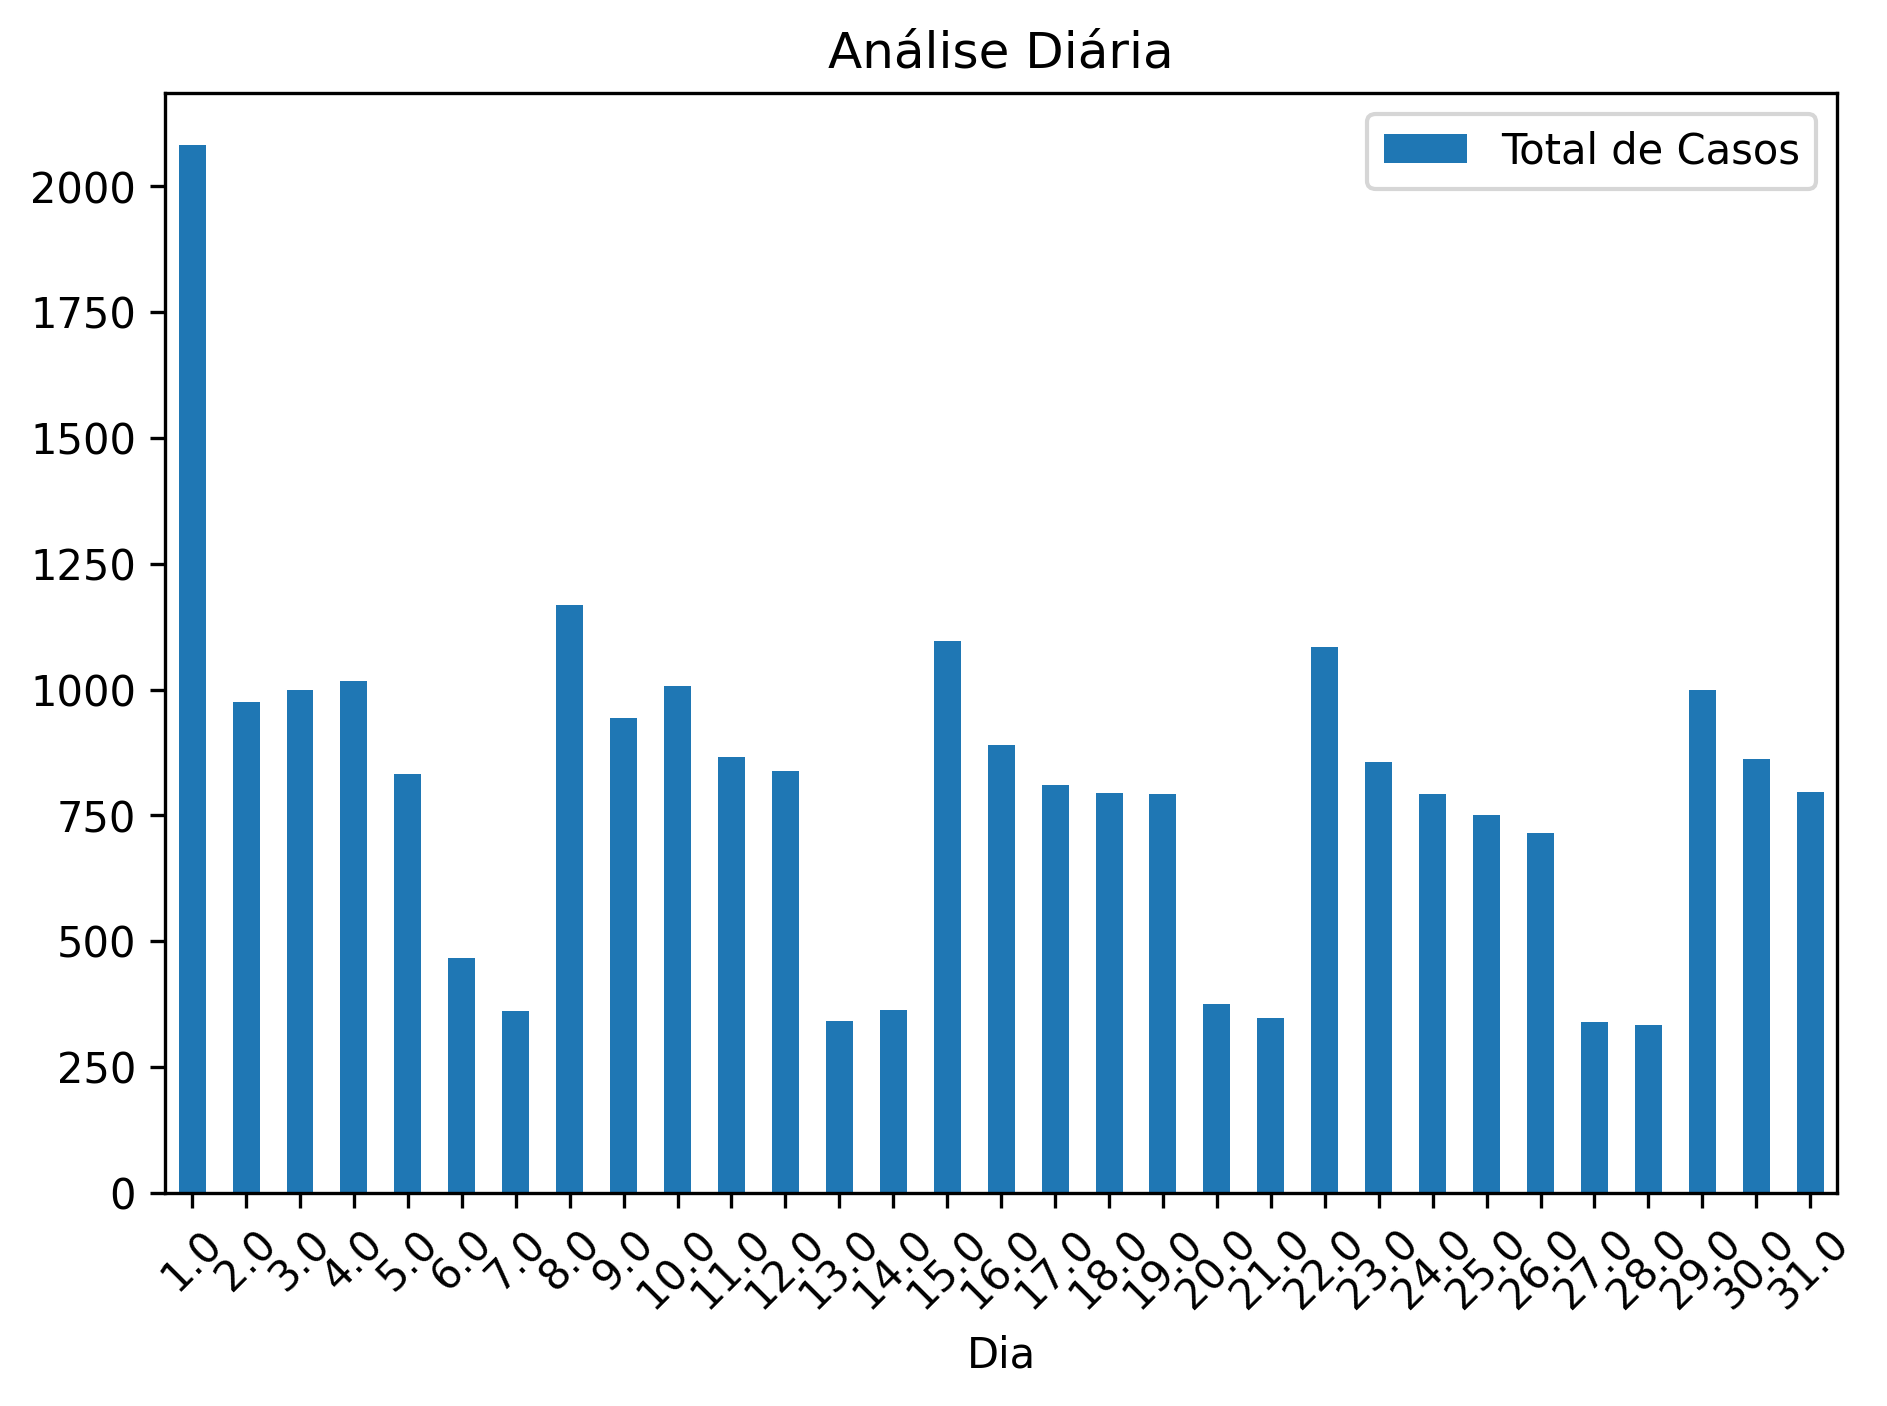
\includegraphics[width=\textwidth]{../graphics/monthly-analysis.png}%
\caption{Análise Mensal}%
\label{fig:casos-30-dias}%
\end{minipage}%
\begin{minipage}{0.45\textwidth}%
\centering%
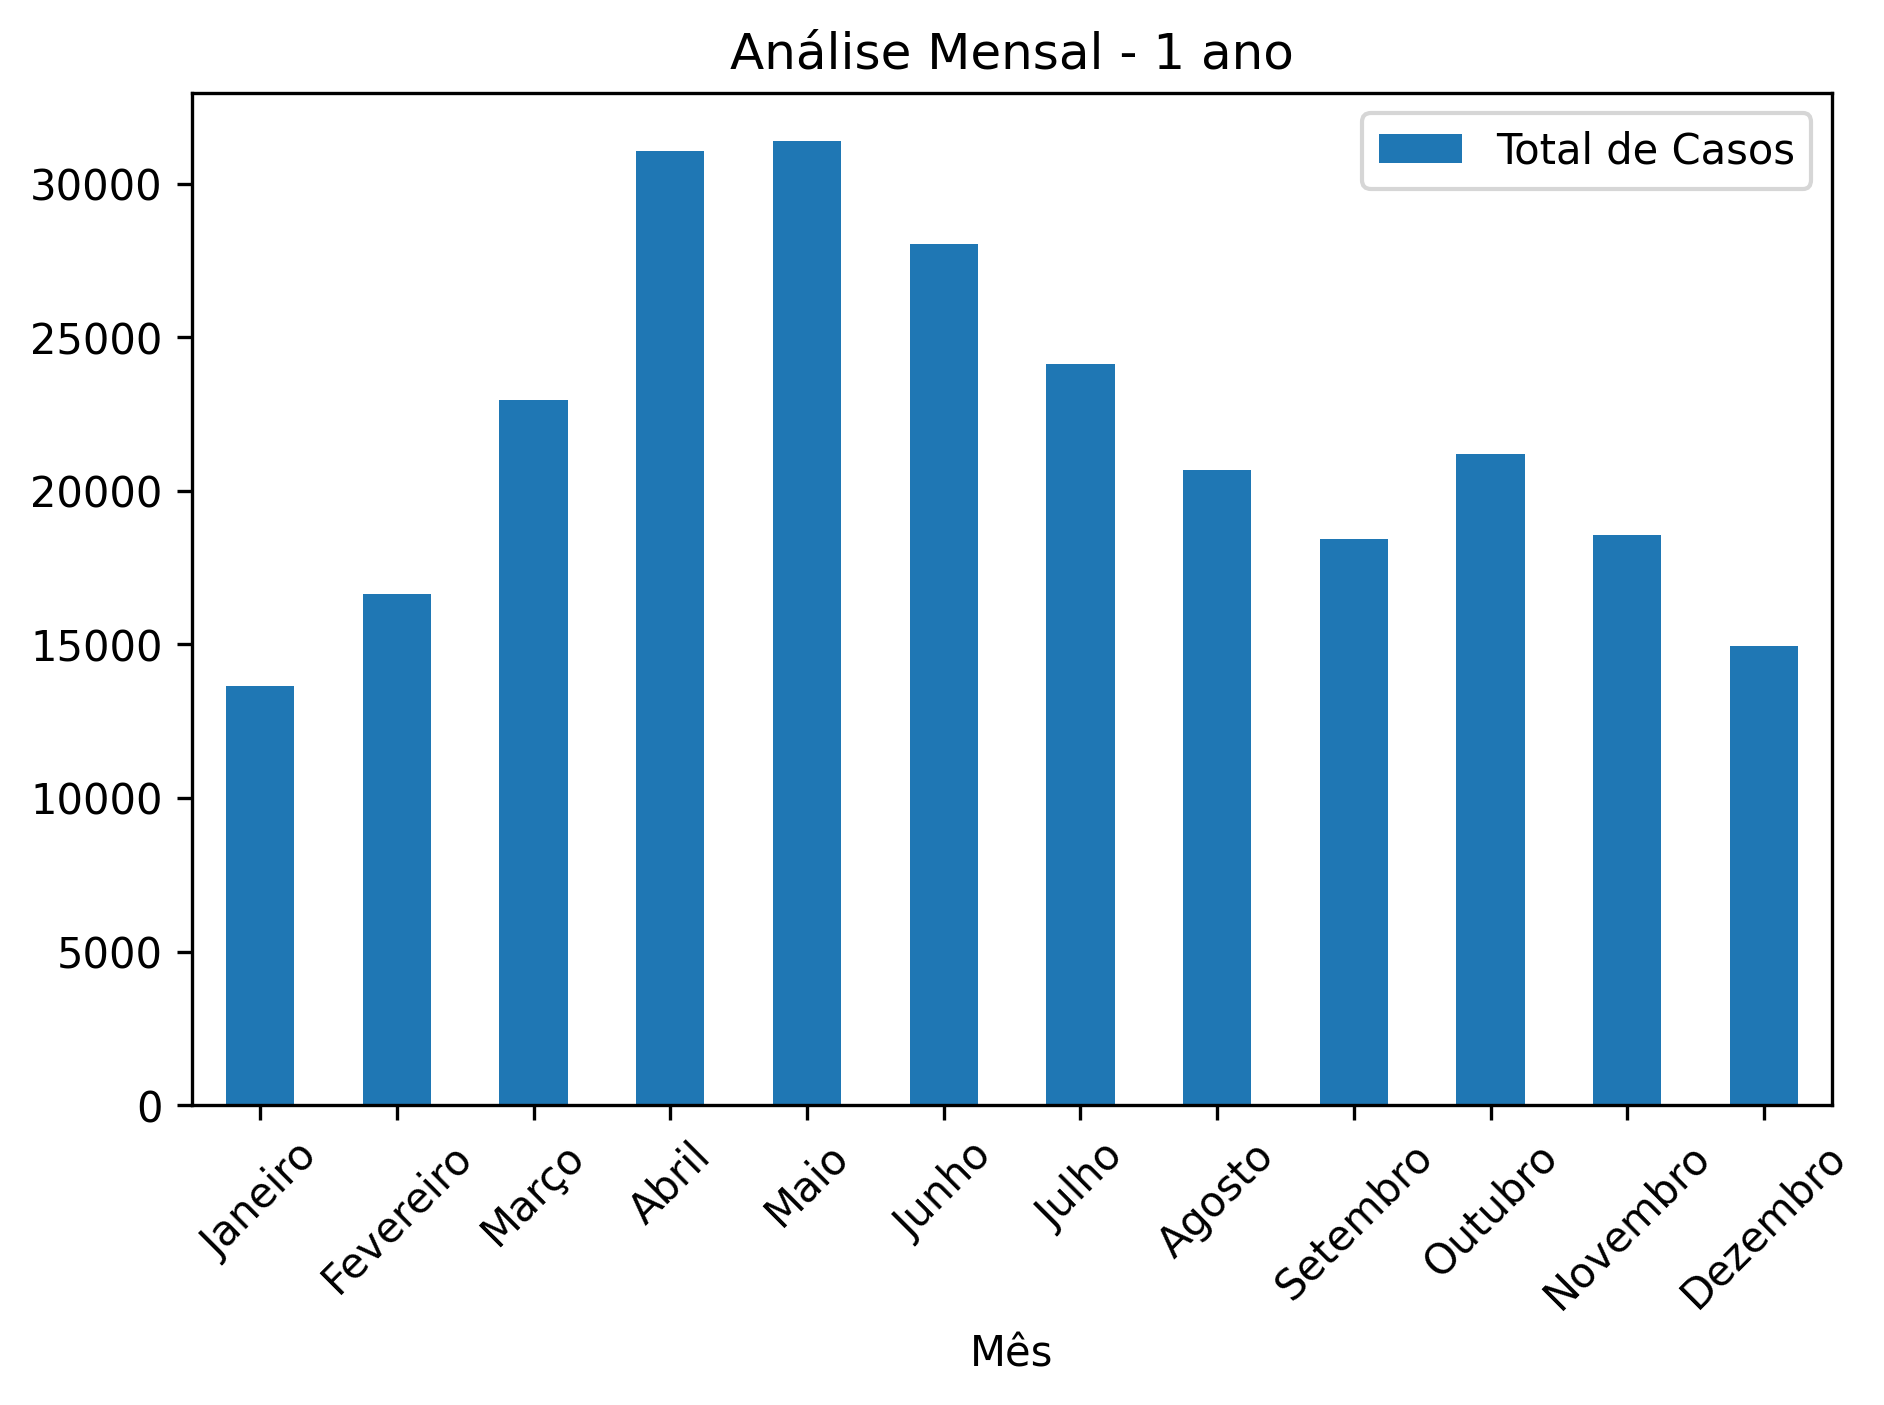
\includegraphics[width=\textwidth]{../graphics/yearly-analysis.png}%
\caption{Análise Anual}%
\label{fig:casos-12-meses}%
\end{minipage}%
\end{figure}

%
\end{document}